\documentclass[tikz]{standalone}
\usepackage{tikz}
\usepackage{setspace}
\usepackage[UTF8]{ctex}
\usetikzlibrary{fit}
\usetikzlibrary{shapes}
\usetikzlibrary{backgrounds} 
\begin{document}
		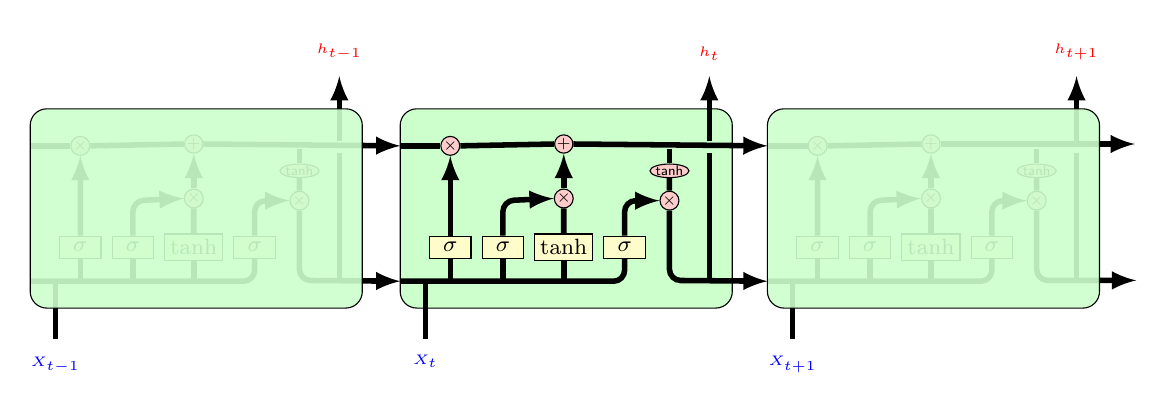
\begin{tikzpicture}[scale=0.9]
			\tikzstyle{layer} = [draw,inner sep=2pt,font=\footnotesize,fill=yellow!20,align=center,minimum width=1.5em,minimum height=0.8em]
			\tikzstyle{point} = [circle,draw,fill=red!20,inner sep=0pt,align=center,font=\tiny]
			\tikzstyle{unit} = [circle,font=\tiny,align=center,inner sep=0pt,align=center,minimum size=1.6em]

			%block 1
			\node[layer] (layer_1) at (0,0) {$\sigma$};
			\node[anchor=west,layer] (layer_2) at ([xshift=0.4em]layer_1.east) {$\sigma$};
			\node[anchor=west,layer] (layer_3) at ([xshift=0.4em]layer_2.east) {tanh};
			\node[anchor=west,layer] (layer_4) at ([xshift=0.4em]layer_3.east) {$\sigma$};
			\node[anchor=south,point] (point_1) at ([yshift=3.2em]layer_1.north) {$\times$};
			\node[anchor=south,point] (point_2) at ([yshift=3.2em]layer_3.north) {+};
    	\node[anchor=south,point] (point_3) at ([yshift=1em]layer_3.north) {$\times$};
    	\node[anchor=south,point] (point_4) at ([xshift=1.8em,yshift=1em]layer_4.north) {$\times$};
			\node[anchor=south,point,ellipse] (point_5) at ([yshift=0.5em]point_4.north) {\textsf{tanh}};
			\node[anchor=north,unit] (xt) at ([xshift=-1em,yshift=-3.2em]layer_1.south){\color{blue}$X_{t}$};
			\node[anchor=south,unit] (ht) at ([xshift=1.6em,yshift=4.6em]point_4.north){\color{red}$h_{t}$};
			
			%block 2
			\node[layer] (layer_1_2) at ([xshift=-14em]layer_1.west) {$\sigma$};
			\node[anchor=west,layer] (layer_2_2) at ([xshift=0.4em]layer_1_2.east) {$\sigma$};
			\node[anchor=west,layer] (layer_3_2) at ([xshift=0.4em]layer_2_2.east) {tanh};
			\node[anchor=west,layer] (layer_4_2) at ([xshift=0.4em]layer_3_2.east) {$\sigma$};
			\node[anchor=south,point] (point_1_2) at ([yshift=3.2em]layer_1_2.north) {$\times$};
			\node[anchor=south,point] (point_2_2) at ([yshift=3.2em]layer_3_2.north) {+};
    	\node[anchor=south,point] (point_3_2) at ([yshift=1em]layer_3_2.north) {$\times$};
    	\node[anchor=south,point] (point_4_2) at ([xshift=1.8em,yshift=1em]layer_4_2.north) {$\times$};
			\node[anchor=south,point,ellipse] (point_5_2) at ([yshift=0.5em]point_4_2.north) {\textsf{tanh}};
			\node[anchor=north,unit] (xt_2) at ([xshift=-1em,yshift=-3.2em]layer_1_2.south){\color{blue}$X_{t-1}$};
			\node[anchor=south,unit] (ht_2) at ([xshift=1.6em,yshift=4.6em]point_4_2.north){\color{red}$h_{t-1}$};
			
			%block 3
			\node[layer] (layer_1_3) at ([xshift=15.6em]layer_1.west) {$\sigma$};
			\node[anchor=west,layer] (layer_2_3) at ([xshift=0.4em]layer_1_3.east) {$\sigma$};
			\node[anchor=west,layer] (layer_3_3) at ([xshift=0.4em]layer_2_3.east) {tanh};
			\node[anchor=west,layer] (layer_4_3) at ([xshift=0.4em]layer_3_3.east) {$\sigma$};
			\node[anchor=south,point] (point_1_3) at ([yshift=3.2em]layer_1_3.north) {$\times$};
			\node[anchor=south,point] (point_2_3) at ([yshift=3.2em]layer_3_3.north) {+};
    	\node[anchor=south,point] (point_3_3) at ([yshift=1em]layer_3_3.north) {$\times$};
    	\node[anchor=south,point] (point_4_3) at ([xshift=1.8em,yshift=1em]layer_4_3.north) {$\times$};
			\node[anchor=south,point,ellipse] (point_5_3) at ([yshift=0.5em]point_4_3.north) {\textsf{tanh}};
			\node[anchor=north,unit] (xt_3) at ([xshift=-1em,yshift=-3.2em]layer_1_3.south){\color{blue}$X_{t+1}$};
			\node[anchor=south,unit] (ht_3) at ([xshift=1.6em,yshift=4.6em]point_4_3.north){\color{red}$h_{t+1}$};
    	
    	%line for block 1
			\draw [-,line width=2pt] ([xshift=-1.6em]point_1.west) -- (point_1.west);
			\draw [-,line width=2pt] (point_1.east) -- (point_2.west);
			\draw [-latex,line width=2pt] (point_2.east) -- ([xshift=-1.6em]point_1_3.west);
			\draw [-,line width=2pt,rounded corners] ([xshift=-2em,yshift=-0.9em]layer_1.south) -- ([yshift=-0.9em]layer_4.south) -- (layer_4.south);
			\draw [-,line width=2pt] ([yshift=-0.9em]layer_1.south) -- (layer_1.south);
			\draw [-latex,line width=2pt] (layer_1.north) -- (point_1.south);
			\draw [-,line width=2pt] ([yshift=-0.9em]layer_2.south) -- (layer_2.south);
			\draw [-,line width=2pt] ([yshift=-0.9em]layer_3.south) -- (layer_3.south);
			\draw [-latex,line width=2pt,rounded corners] (layer_2.north) -- ([yshift=1.4em]layer_2.north) -- (point_3.west);
			\draw [-,line width=2pt] (layer_3.north) -- (point_3.south);
			\draw [-latex,line width=2pt] (point_3.north) -- (point_2.south);
			\draw [-latex,line width=2pt,rounded corners] (layer_4.north) -- ([yshift=1.4em]layer_4.north) -- (point_4.west);
			\draw [-,line width=2pt] ([yshift=0.6em]point_5.north) -- (point_5.north);
			\draw [-,line width=2pt] (point_5.south) -- (point_4.north);
			\draw [-latex,line width=2pt,rounded corners] (point_4.south) -- ([yshift=-2.8em]point_4.south) -- ([xshift=-2em,yshift=-0.9em]layer_1_3.south);
			\draw [-latex,line width=2pt] ([yshift=-2.6em]ht.south) -- (ht.south);
			\draw [-,line width=2pt] ([yshift=-8.2em]ht.south) -- ([yshift=-3.1em]ht.south);
			\draw [-,line width=2pt] (xt.north) -- ([yshift=2.2em]xt.north);
			
			%line for block 2
			\draw [-,line width=2pt] ([xshift=-1.6em]point_1_2.west) -- (point_1_2.west);
			\draw [-,line width=2pt] (point_1_2.east) -- (point_2_2.west);
			\draw [-latex,line width=2pt] (point_2_2.east) -- ([xshift=-1.6em]point_1.west);
			\draw [-,line width=2pt,rounded corners] ([xshift=-2em,yshift=-0.9em]layer_1_2.south) -- ([yshift=-0.9em]layer_4_2.south) -- (layer_4_2.south);
			\draw [-,line width=2pt] ([yshift=-0.9em]layer_1_2.south) -- (layer_1_2.south);
			\draw [-latex,line width=2pt] (layer_1_2.north) -- (point_1_2.south);
			\draw [-,line width=2pt] ([yshift=-0.9em]layer_2_2.south) -- (layer_2_2.south);
			\draw [-,line width=2pt] ([yshift=-0.9em]layer_3_2.south) -- (layer_3_2.south);
			\draw [-latex,line width=2pt,rounded corners] (layer_2_2.north) -- ([yshift=1.4em]layer_2_2.north) -- (point_3_2.west);
			\draw [-,line width=2pt] (layer_3_2.north) -- (point_3_2.south);
			\draw [-latex,line width=2pt] (point_3_2.north) -- (point_2_2.south);
			\draw [-latex,line width=2pt,rounded corners] (layer_4_2.north) -- ([yshift=1.4em]layer_4_2.north) -- (point_4_2.west);
			\draw [-,line width=2pt] ([yshift=0.6em]point_5_2.north) -- (point_5_2.north);
			\draw [-,line width=2pt] (point_5_2.south) -- (point_4_2.north);
			\draw [-latex,line width=2pt,rounded corners] (point_4_2.south) -- ([yshift=-2.8em]point_4_2.south) -- ([xshift=-2em,yshift=-0.9em]layer_1.south);
			\draw [-latex,line width=2pt] ([yshift=-2.6em]ht_2.south) -- (ht_2.south);
			\draw [-,line width=2pt] ([yshift=-8.2em]ht_2.south) -- ([yshift=-3.1em]ht_2.south);
			\draw [-,line width=2pt] (xt_2.north) -- ([yshift=2.2em]xt_2.north);
			
			%line for block 3
			\draw [-,line width=2pt] ([xshift=-1.6em]point_1_3.west) -- (point_1_3.west);
			\draw [-,line width=2pt] (point_1_3.east) -- (point_2_3.west);
			\draw [-latex,line width=2pt] (point_2_3.east) -- ([xshift=7.8em]point_2_3.east);
			\draw [-,line width=2pt,rounded corners] ([xshift=-2em,yshift=-0.9em]layer_1_3.south) -- ([yshift=-0.9em]layer_4_3.south) -- (layer_4_3.south);
			\draw [-,line width=2pt] ([yshift=-0.9em]layer_1_3.south) -- (layer_1_3.south);
			\draw [-latex,line width=2pt] (layer_1_3.north) -- (point_1_3.south);
			\draw [-,line width=2pt] ([yshift=-0.9em]layer_2_3.south) -- (layer_2_3.south);
			\draw [-,line width=2pt] ([yshift=-0.9em]layer_3_3.south) -- (layer_3_3.south);
			\draw [-latex,line width=2pt,rounded corners] (layer_2_3.north) -- ([yshift=1.4em]layer_2_3.north) -- (point_3_3.west);
			\draw [-,line width=2pt] (layer_3_3.north) -- (point_3_3.south);
			\draw [-latex,line width=2pt] (point_3_3.north) -- (point_2_3.south);
			\draw [-latex,line width=2pt,rounded corners] (layer_4_3.north) -- ([yshift=1.4em]layer_4_3.north) -- (point_4_3.west);
			\draw [-,line width=2pt] ([yshift=0.6em]point_5_3.north) -- (point_5_3.north);
			\draw [-,line width=2pt] (point_5_3.south) -- (point_4_3.north);
			\draw [-latex,line width=2pt,rounded corners] (point_4_3.south) -- ([yshift=-2.8em]point_4_3.south) -- ([xshift=4em,yshift=-2.8em]point_4_3.south);
			\draw [-latex,line width=2pt] ([yshift=-2.6em]ht_3.south) -- (ht_3.south);
			\draw [-,line width=2pt] ([yshift=-8.2em]ht_3.south) -- ([yshift=-3.1em]ht_3.south);
			\draw [-,line width=2pt] (xt_3.north) -- ([yshift=2.2em]xt_3.north);
			
			%background
			\begin{pgfonlayer}{background}
       	\node[rectangle,draw,fill=green!20,rounded corners=6pt,minimum width=12em,minimum height=7.2em] at ([xshift=0.1em,yshift=-0.4em]point_3) (box0) {};
    	\end{pgfonlayer}
    	\node[rectangle,fill opacity=0.9,draw,fill=green!20,rounded corners=6pt,minimum width=12em,minimum height=7.2em] at ([xshift=0.1em,yshift=-0.4em]point_3_2) (box1) {};
      \node[rectangle,fill opacity=0.9,draw,fill=green!20,rounded corners=6pt,minimum width=12em,minimum height=7.2em] at ([xshift=0.1em,yshift=-0.4em]point_3_3) (box2) {};
		\end{tikzpicture}
\end{document} 